\subsubsection{Types}
Service calls usually return data in JSON format. Javascript\textsubscript{G} and Typescript\textsubscript{G} are able to convert JSON\textsubscript{G} format into a class object.\\
Because of this, the \textit{EmporioLambda} Front-end\textsubscript{G} module uses many not-primitive interfaces and classes in order to correctly convert the received JSON\textsubscript{G} data. These classes can be found inside the \textit{src/types} folder. To send data, you can use the JSON.stringify function which converts an object passed as parameter into a JSON\textsubscript{G} format string.\\Here's a class diagram that shows these classes and their dependencies between each other:
\vspace{0.5cm}
\begin{figure}[H]
\centering
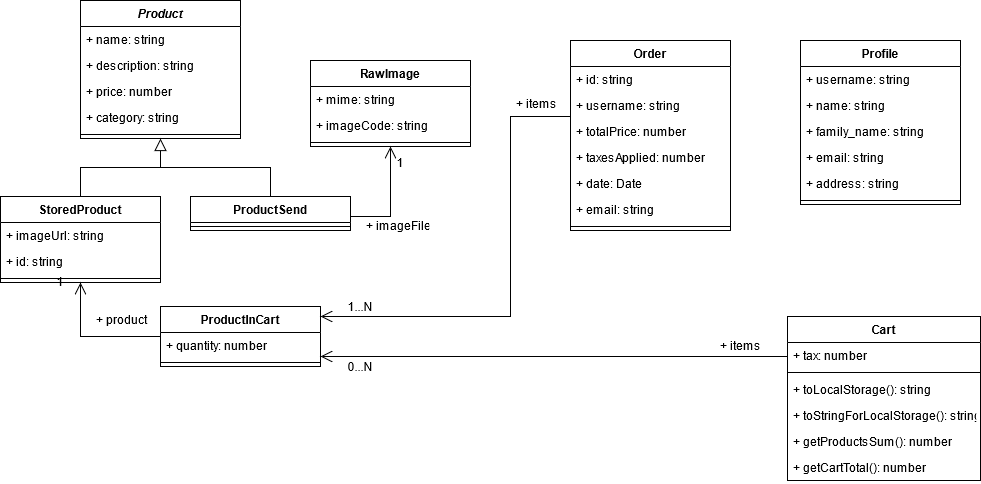
\includegraphics[scale=0.45]{res/Architettura/Frontend/img/class_frontend_types}\\
\caption{Diagram of the classes and types used in the Front-end\textsubscript{G} module}
\end{figure}